\documentclass{beamer}

\beamertemplatenavigationsymbolsempty
\usetheme{Warsaw}

\title{Computer Graphics -- Homework 2}
\author{Tran Phong Binh}
\institute{Student ID: 110062421}
\date{\today}

\begin{document}

\begin{frame}
  \titlepage
\end{frame}

\begin{frame}
  \frametitle{Executable}
  \begin{itemize}
    \item The shaders must be in the same folder as the binary's in order to execute the program.
  \end{itemize}
  \begin{figure}
    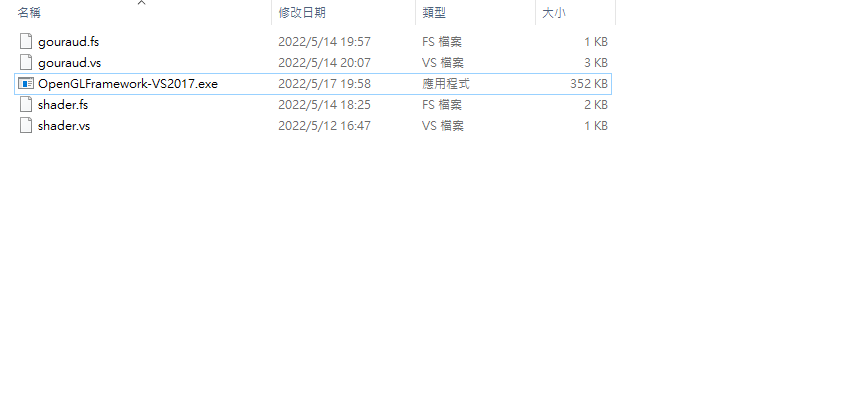
\includegraphics[width=\textwidth]{executable}
    \caption{Executable folder}
  \end{figure} 
\end{frame}

\begin{frame}
  \frametitle{Static Key Controls}
  \begin{itemize}
    \item Z: previous model
    \item X: next model
    \item L: directional/point/spot light
  \end{itemize}
\end{frame}

\begin{frame}
  \frametitle{Dynamic Key Controls}
  In the modes below, x-, y-, and z-axis are modified according to mouse's horizontal drag, vertical drag, and scrolling, respectively.
  \begin{itemize}
    \item T: model translation
    \item R: model rotation
    \item S: model scaling
    \item K: light editing
    \item J: shininess editing
  \end{itemize}
\end{frame}

\begin{frame}
  \frametitle{Special Key Control}
  \begin{itemize}
    \item W: solid/wireframe
  \end{itemize}
  \begin{figure}
    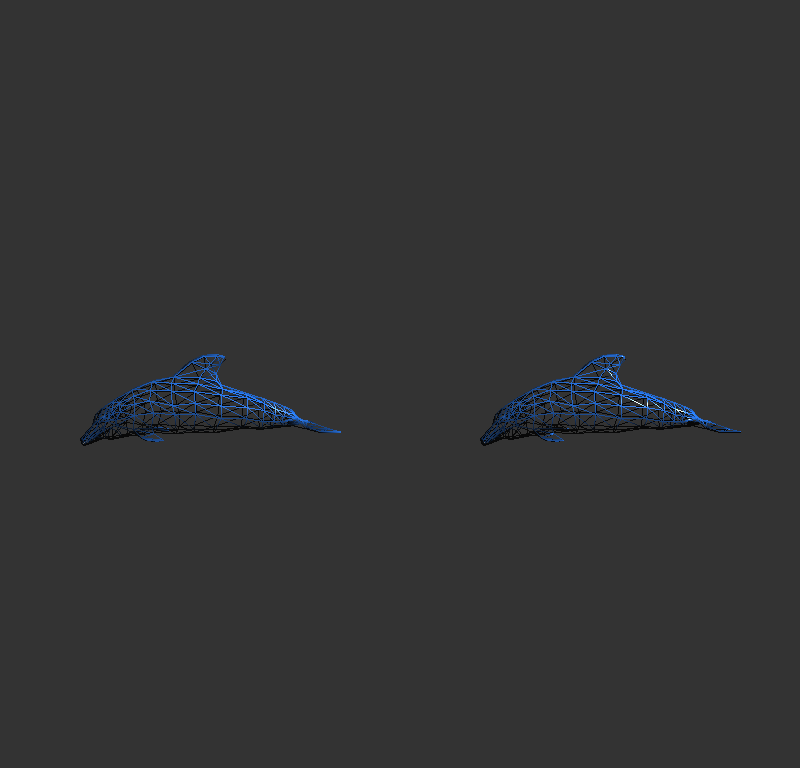
\includegraphics[width=0.5\textwidth]{wireframe}
    \caption{Wireframe}
  \end{figure}
\end{frame}

\begin{frame}
  \frametitle{Model TRS}
  \begin{figure}
    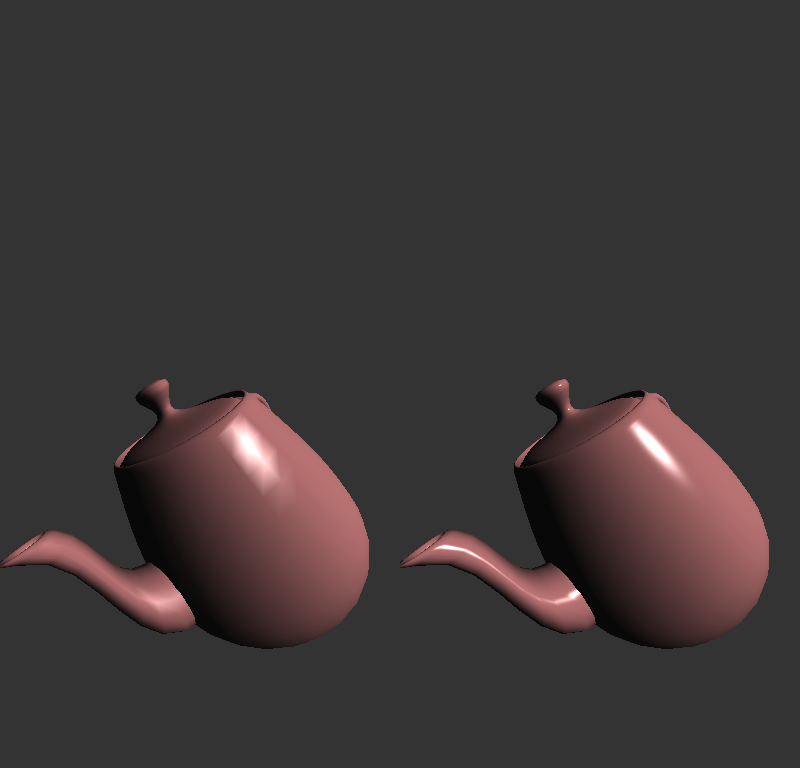
\includegraphics[width=0.5\textwidth]{model_trs}
    \caption{Model translation, rotation, and scaling}
  \end{figure}
\end{frame}

\begin{frame}
  \frametitle{Light Editing}
  \begin{figure}
    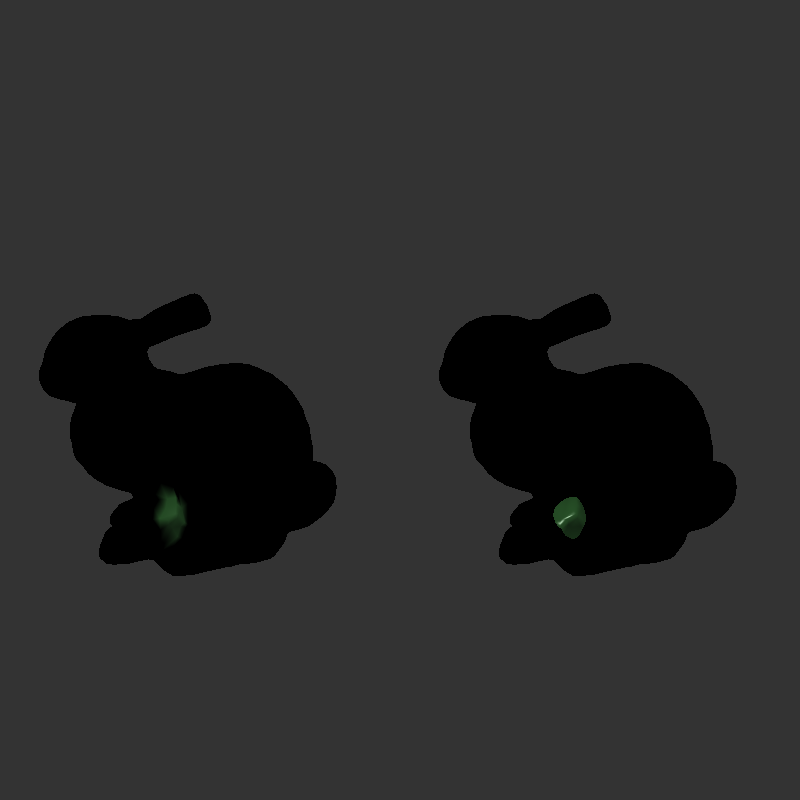
\includegraphics[width=0.5\textwidth]{light_edit}
    \caption{Spot light editing}
  \end{figure}
\end{frame}

\begin{frame}
  \frametitle{Shininess Editing}
  \begin{figure}
    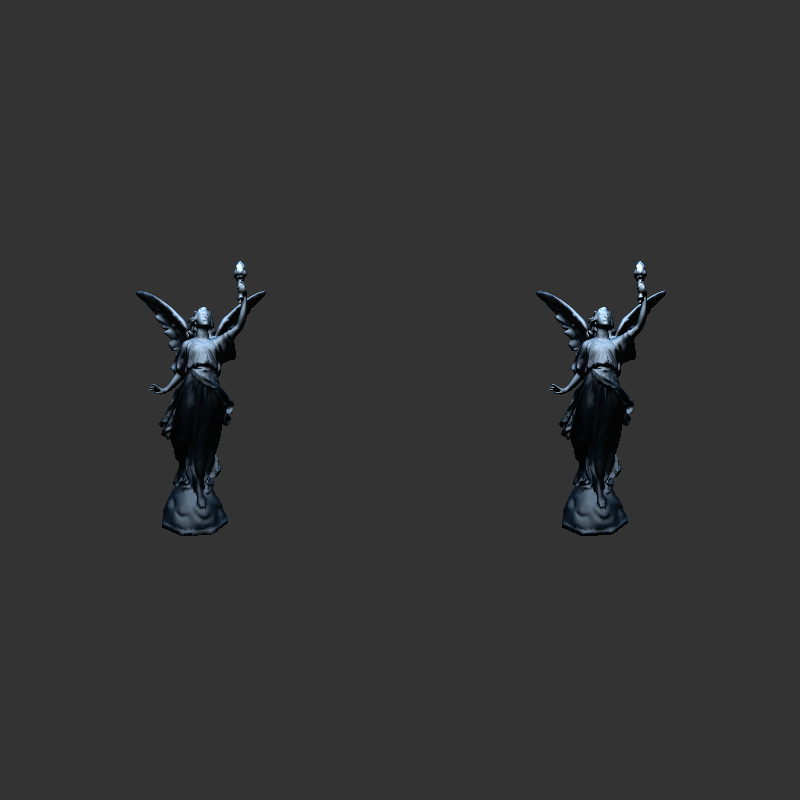
\includegraphics[width=0.5\textwidth]{shininess}
    \caption{Point light shininess editing}
  \end{figure}
\end{frame}

\end{document}
